\input sys/inputs.tex

\begin{document}

\bigheading{Plakáty na zdi}

% \info{task_name}{infile}{outfile}{points}{timelimit}{memlimit}
% leave this values, if you are not interested
\info{posters}{stdin}{stdout}{100}{2000 ms}{1 GB}

V tajné základně Kamarádů svatých postulátů se nachází Stěna. Na Stěně visí
plakáty s přísně střeženými a hlavně nebezpečnými tajemstvími vesmíru. Aby se
však předešlo katastrofám a nechtěným následkům, plakáty se nepřekrývají (mohou
se však dotýkat).

Jednou za čas přijde nová várka plakátů, které zasluhují zavěšení na Stěně.
Kamarádi se při této vzácné příležitosti potýkají s obzvlášť těžkým a závažným
problémem: Kam pověsit nové plakáty? Naštěstí mají osvědčený postup, kterým se
řídí. Naneštěstí je tento postup příliš komplikovaný. Vaší úlohou bude pomoci
s jedním krokem tohoto postupu.

Momentálně se pro nové plakáty vybírají slibné pozice. Pro mnoho pozic různých
plakátů rychle spočítejte plochu původních plakátů, která byla zakrytá daným
umístěním nového plakátu.

\heading{Úloha}

Dostanete popis $n$ nepřekrývajících se šedých obdélníků v bílé rovině. Dále
dostanete $q$ dotazů na zpracování ve tvaru: Jaký je obsah šedé plochy
v zananém obdélníku? Pozor, tímto \textbf{nepřidáváme} nový obdélník do plochy.

Odpověď zpracujte online.

\heading{Vstup}

Na prvním řádku dostanete pět čísel $r, c, n, q, m$, ($1 \leq r, c < m \leq 10^9 + 9$, $0 \leq n,q \leq 50\,000$),
šířku a výšku Stěny, počet plakátů na Stěně, počet dotazů a speciální modulus na
počítání dotazů (ten vysvětlíme později).

Na každém z následujících $n$ řádků budou čtyři čísla, $x_1, y_1, x_2, y_2$ ($0 \leq x_1, x_2 \leq r$,
$0 \leq y_1, y_2 \leq c$), souřadnice dvou protilehlých bodů obdélníku.

Následuje $q$ řádků, v každém z nich je pět čísel $x_1^*, y_1^*, x_2^*, y_2^*, v$
v rozsahu od $0$ do $m - 1$ včetně. Z těchto čísel vypočítejte reálné souřadnice
dotazovaného obdélníku pomocí vzorce dole.

Označme $l$ jako odpověď na předešlý dotaz (pro úplně první dotaz položíme $l=0$). Potom
$$x_i = (x_i^* + l \cdot v) \pmod m$$
$$y_i = (y_i^* + l \cdot v) \pmod m$$

Dekódované souřadnice $x_1, y_1, x_2, y_2$ splňující následující podmínky:
$0 \leq x_1, x_2 \leq r$, $0 \leq y_1, y_2 \leq c$. 

\heading{Výstup}

Pro každý dotaz vypište jeden řádek obsahující jediné číslo: odpověď na dotaz.

\heading{Podproblémy}

Úloha má vícero podúloh. V offline podúlohách bude hodnota $v$ vždy nulová.

\bigskip

\begin{center}
\begin{tabular}{|l|l|l|l|l|l|}
\hline
podproblém & body & nejvyšší $r$  & nejvyšší $c$   & nejvyšší $n$ a $q$ & online    \\ \hline
1       & 10     & $500$        & $500$         & $500$     & ne        \\ \hline
2       & 10     & $5000$       & $5000$        & $5000$    & ne        \\ \hline
3       & 40     & $300\,000$   & $300\,000$    & $50\,000$ & ne        \\ \hline
4       & 10     & $10^9$       & $200\,000$    & $50\,000$ & ne        \\ \hline
5       & 10     & $10^9$       & $10^9$        & $50\,000$ & ne        \\ \hline
6       & 10     & $100\,002$   & $100\,002$    & $50\,000$ & ano       \\ \hline
7       & 10     & $10^9 + 8$   & $10^9 + 8$    & $50\,000$ & ano       \\ \hline
\end{tabular}
\end{center}

\heading{Příklady}


\sampleIN
8 11 3 4 13
1 1 5 5
7 7 5 4
4 6 2 7
1 1 7 8 0
2 2 4 3 0
3 4 6 7 0
2 9 3 10 0
\sampleOUT
24
2
6
0
\sampleCOMMENT
Tento případ si můžete prohlédnout na obrázku níže.
\sampleEND
\center{
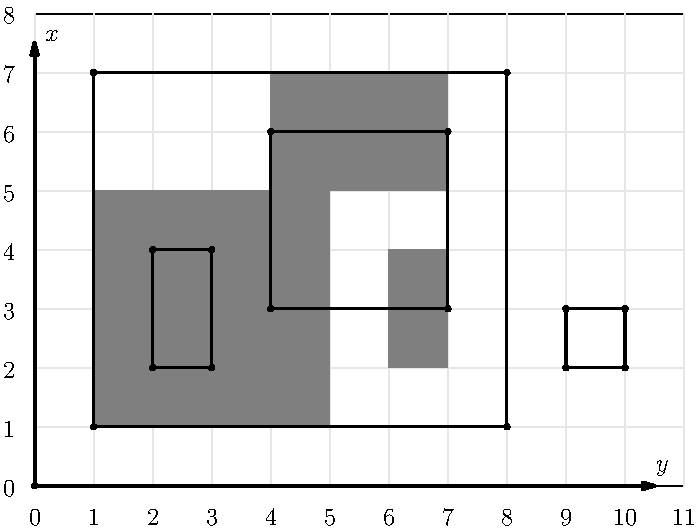
\includegraphics[width=12cm]{img/posters.pdf}
}

\sampleIN
8 11 3 4 13
1 1 5 5
7 7 5 4
4 6 2 7
1 1 7 8 4
6 6 8 7 2
2 3 5 6 7
11 5 12 6 5
\sampleOUT
24
2
6
0
\sampleCOMMENT
Toto je stejný vstup jako výše s využitím online dotazů.
\sampleEND
\end{document}
